\documentclass{article}[18pt]
\usepackage{../../../../format}
\lhead{Programming Paradigms - Functional Programming}
\usepackage{minted}
\setminted{tabsize=4}
\usetikzlibrary{trees}
\begin{document}
\begin{center}
\underline{\huge Lazy evaluation}
\end{center}
\section{Lazy Evaluation}
\begin{itemize}
	\item Not only is Haskell a pure functional language
	\item It is also evaluated lazily
	\item Hence, we can work with infinite data structures
	\item And defer computation until such time as it's strictly necessary
\end{itemize}
\begin{defin}[Lazy evaluation]
Expressions are not evaluated when they are bound to variables. Instead, their evaluation is deferred until their result is needed by other computations
\end{defin}
\subsection{Evaluation strategies}
\begin{itemize}
	\item Haskell's basic method of computation is an application of functions to arguments
	\item Even here, though we already have some freedom
\end{itemize}
\begin{minted}{haskell}
inc :: Int -> Int
inc n = n + 1
inc (2+3)
\end{minted}
\begin{minipage}{0.5\textwidth}
\begin{minted}{haskell}
inc (2+3)
= inc 6 -- applying *
= 6 + 1 -- applying inc
= 7 -- applying *
\end{minted}
\end{minipage}
\begin{minipage}{0.5\textwidth}
\begin{minted}{haskell}
inc (2+3)
= (2*3) + 1 -- applying inc
= 6 + 1 -- applying *
= 7 -- applying +
\end{minted}
\end{minipage}
\begin{itemize}
	\item As long as all expression evaluations terminate, the order we choose to do things doesn't matter
	\item We can represent a function call and its arguments as a graph
	\item Nodes in the graph are either terminal or compound. The latter are called reducible expressions or redexes
\end{itemize}


\begin{minipage}{0.5\textwidth}
\begin{minted}{haskell}
mult :: (Int, Int) -> Int
mult (x, y) = x*y
mult (1+2, 3+4)
\end{minted}
\end{minipage}
\begin{minipage}{0.5\textwidth}
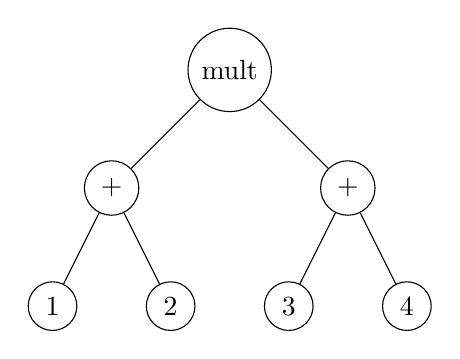
\begin{tikzpicture}[level distance=1.5cm,
level 1/.style={sibling distance=3cm},
level 2/.style={sibling distance=1.5cm}]
\node[circle,draw] {mult}
child {node[circle,draw] {+}
	child {node[circle,draw] {1}}
	child {node[circle,draw] {2}}
}
child {node[circle,draw] {+}
	child {node[circle,draw] {3}}
	child {node[circle,draw] {4}}
};
\end{tikzpicture}
\end{minipage}

\begin{itemize}
	\item 1,2,3, and 4 are terminal (not reducible) expressions
	\item (+) and milt are reducible expressions
\end{itemize}
\subsubsection{Innermost evaluation}
\begin{itemize}
	\item Evaluate "bottom up"
	\item First evaluate redexes that only contain terminal or irreducible expressions, then repeat
	\item Need to specify evaluation order at leaves. Typically : "left to right"
\end{itemize}
\begin{minipage}{0.2\textwidth}
	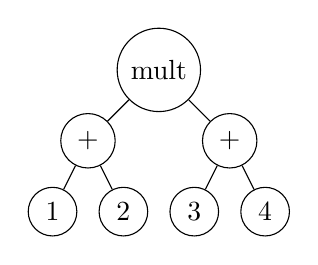
\begin{tikzpicture}[level distance=1.5cm,
	level 1/.style={sibling distance=3cm},
	level 2/.style={sibling distance=1.5cm},scale=0.6]
	\node[circle,draw] {mult}
	child {node[circle,draw] {+}
		child {node[circle,draw] {1}}
		child {node[circle,draw] {2}}
	}
	child {node[circle,draw] {+}
		child {node[circle,draw] {3}}
		child {node[circle,draw] {4}}
	};
	\end{tikzpicture}
\end{minipage}
\begin{minipage}{0.2\textwidth}
	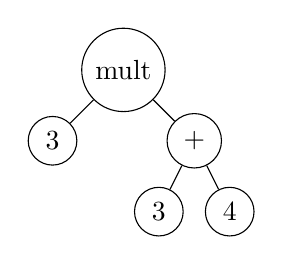
\begin{tikzpicture}[level distance=1.5cm,
	level 1/.style={sibling distance=3cm},
	level 2/.style={sibling distance=1.5cm},scale=0.6]
	\node[circle,draw] {mult}
	child {node[circle,draw] {3}}
	child {node[circle,draw] {+}
		child {node[circle,draw] {3}}
		child {node[circle,draw] {4}}
	};
	\end{tikzpicture}
\end{minipage}
\begin{minipage}{0.2\textwidth}
	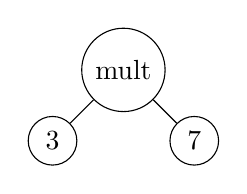
\begin{tikzpicture}[level distance=1.5cm,
	level 1/.style={sibling distance=3cm},
	level 2/.style={sibling distance=1.5cm},scale=0.6]
	\node[circle,draw] {mult}
	child {node[circle,draw] {3}}
	child {node[circle,draw] {7}};
	\end{tikzpicture}
\end{minipage}
\begin{minipage}{0.2\textwidth}
	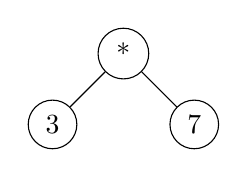
\begin{tikzpicture}[level distance=1.5cm,
	level 1/.style={sibling distance=3cm},
	level 2/.style={sibling distance=1.5cm},scale=0.6]
	\node[circle,draw] {*}
	child {node[circle,draw] {3}}
	child {node[circle,draw] {7}};
	\end{tikzpicture}
\end{minipage}
\begin{minipage}{0.2\textwidth}
	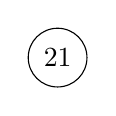
\begin{tikzpicture}[level distance=1.5cm,
	level 1/.style={sibling distance=3cm},
	level 2/.style={sibling distance=1.5cm},scale=0.6]
	\node [circle,draw] {21};
	\end{tikzpicture}
\end{minipage}
\subsubsection{Outermost Evaluation}
\begin{itemize}
	\item Evaluate "top down"
	\item First evaluate redexes that are outermost, then repeat
	\item Again, need an evaluation order for children, typically choose "left to right"
\end{itemize}
\begin{minipage}{0.2\textwidth}
	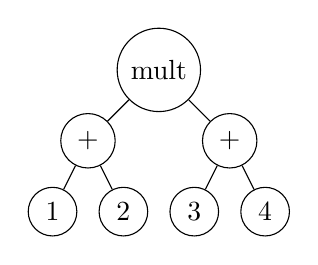
\begin{tikzpicture}[level distance=1.5cm,
	level 1/.style={sibling distance=3cm},
	level 2/.style={sibling distance=1.5cm},scale=0.6]
	\node[circle,draw] {mult}
	child {node[circle,draw] {+}
		child {node[circle,draw] {1}}
		child {node[circle,draw] {2}}
	}
	child {node[circle,draw] {+}
		child {node[circle,draw] {3}}
		child {node[circle,draw] {4}}
	};
	\end{tikzpicture}
\end{minipage}
\begin{minipage}{0.2\textwidth}
	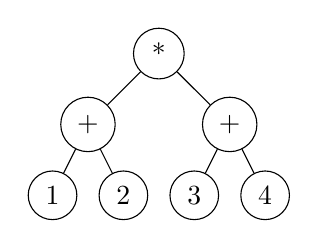
\begin{tikzpicture}[level distance=1.5cm,
	level 1/.style={sibling distance=3cm},
	level 2/.style={sibling distance=1.5cm},scale=0.6]
	\node[circle,draw] {*}
	child {node[circle,draw] {+}
		child {node[circle,draw] {1}}
		child {node[circle,draw] {2}}
	}
	child {node[circle,draw] {+}
		child {node[circle,draw] {3}}
		child {node[circle,draw] {4}}
	};
	\end{tikzpicture}
\end{minipage}
\begin{minipage}{0.2\textwidth}
	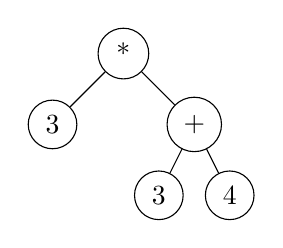
\begin{tikzpicture}[level distance=1.5cm,
	level 1/.style={sibling distance=3cm},
	level 2/.style={sibling distance=1.5cm},scale=0.6]
	\node[circle,draw] {*}
	child {node[circle,draw] {3}}
	child {node[circle,draw] {+}
		child {node[circle,draw] {3}}
		child {node[circle,draw] {4}}
	};
	\end{tikzpicture}
\end{minipage}
\begin{minipage}{0.2\textwidth}
	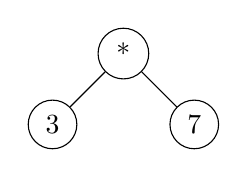
\begin{tikzpicture}[level distance=1.5cm,
	level 1/.style={sibling distance=3cm},
	level 2/.style={sibling distance=1.5cm},scale=0.6]
	\node[circle,draw] {*}
	child {node[circle,draw] {3}}
	child {node[circle,draw] {7}};
	\end{tikzpicture}
\end{minipage}
\begin{minipage}{0.2\textwidth}
	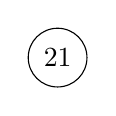
\begin{tikzpicture}[level distance=1.5cm,
	level 1/.style={sibling distance=3cm},
	level 2/.style={sibling distance=1.5cm},scale=0.6]
	\node [circle,draw] {21};
	\end{tikzpicture}
\end{minipage}
\subsection{Termination}
\begin{itemize}
	\item For finite expressions, both innermost and outermost evaluation terminate
	\item Not so for infinite expressions
\end{itemize}
\subsection{Call by name or value}
\begin{minipage}{0.45\textwidth}
\underline{Call by value}
\begin{itemize}
	\item Also called eager evaluation
	\item Innermost evaluation
	\item Arguments to functions are always fully evaluated before the function is applied
	\item Each argument is evaluated exactly once
	\item Evaluation strategy for most imperative languages
\end{itemize}
\end{minipage}
\begin{minipage}{0.1\textwidth}
$ $
\end{minipage}
\begin{minipage}{0.45\textwidth}
\underline{Call by name}
\begin{itemize}
	\item Also called lazy evaluation
	\item Outermost evaluation
	\item Functions are applied before their arguments are evaluated
	\item Each argument may be evaluated more than once
	\item Evaluation strategy in haskell (and others)
\end{itemize}
\end{minipage}
\subsection{Avoiding inefficiencies: sharing}
\begin{itemize}
	\item Straightforward implementation of call-by-name can lead to inefficiency in the number of times an argument is evaluated
\end{itemize}
\begin{minted}{haskell}
square :: Int -> Int
square n = n * n
Prelude> square (1+2)
== (1 + 2) * (1 + 2) -- applying square
== 3 * (1 + 2) -- applying +
== 3 * 3 -- applying +
== 9
\end{minted}
\begin{itemize}
	\item To avoid this, Haskell implements sharing of arguments
	\item We can think of this as rewriting the evaluation tree into a graph
\end{itemize}
\section{Controlling evaluation order}
\begin{defin}[Normal form]
The expression graph contains no redexes, is finite, and is acyclic\\
Data constructors are not reducible, so they "look like functions, there is no reduction rule
\end{defin}
\begin{defin}[Weak head normal form (WHNF)]
The expression graph is in normal form, or the topmost node in the expression graph is a constructor.\\
This allows for cycles
\end{defin}
\subsection{Evaluation rule}
\begin{itemize}
	\item Apply reduction rules (functions) outermost first
	\item Evaluate children "left to right"
	\item Stop when the expression graph is in WHNFF
	\item Function definitions introduce new reduction rules
\end{itemize}
\subsection{Lazy evaluation in strict languages}
\begin{itemize}
	\item All (probably) languages have one place where they do something akin to lazy evaluation
	\item Boolean expressions to short circuit evaluation
	\item Avoids evaluating unnecessary expressions
	\item But not possible when assigning to variables
	\item Python generators are lazily evaluated
	\item Somewhat painful to work with when combining them
\end{itemize}
\subsection{Strict functions}
\begin{defin}[Strict function]
A function which requires its arguments to be evaluated before being applied\\
Even when using outermost evaluation
\end{defin}
Some functions in Haskell are strict (normally when working with numeric types)
\subsubsection{Saving space}
\begin{itemize}
	\item Haskell uses lazy evaluation by default
	\item It also provides a mechanism for strict function application, using the operator (\textdollar!)
\begin{minted}{haskell}
($!) :: (a -> b) -> a -> b
f $! x -- evaluate x then apply f
\end{minted}
	\item When using \textdollar !, the evaluation of the argument is forced until it is in weak head normal form
\begin{minted}{haskell}
square $! (1 + 2)
== square $1 3 -- applying +
== square 3 -- applying $!
== 3*3 -- applying square
== 9 -- applying *
\end{minted}
	\item This allows us to write functions that evaluate as if we had call-by-value semantics, rather than the default call-by-name
	\item Lazy evaluation can require a large amount of space to generate the expression graph
	\item In contrast, strict evaluation always evaluates the summation immediately, using constant space
	\item This kind of strict evaluation can be useful
	\item \mintinline{haskell}{sumwith} is "just" a tail recursive left fold
\begin{minted}{haskell}
sumwith  = foldl (+) 0
\end{minted}
	\item For a strict version, which uses less space, we can use \mintinline{haskell}{foldl'}
\begin{minted}{haskell}
import Data.Foldable
sumwith' = foldl' (+) 0
\end{minted}
	\item This can have reasonable time saving for large expressions
\end{itemize}
\end{document}